% !TEX root = ../main.tex

%************************************************
\chapter{Outflows and hot dust emission}
\label{ch:sed} 

% Refer to: 
% HotDustPaper/
 % summary-150309.ipynb
 % notes.md
 % correlations_summary_141204.ipynb
 % correlations_summary.md
 % various *.md 

%************************************************

\section{Introduction}

Many quasars and AGNs show an excess in their near-infrared continuum emission. 
This feature is generally attributed to thermal emission from dust heated by optical/ultraviolet radiation from the accretion disc. 
The wavelength of the feature ($\sim2$\,$\mu$m) corresponds to the spectral peak for graphite dust at its sublimation temperature \citep[${\mathrm T}\sim1500$\,K;][]{barvainis87}. 
Reverberation measurements of nearby AGNs suggest that the hot dust is very close to the central source \citep[few tens of light days; e.g.][]{minezaki04,suganuma06}.
This places the dust at the innermost edge of the putative torus-like structure, at a radius set by the sublimation temperature of the dust grains.  

Studies have fitted the near-infrared SEDs of AGNs using a blackbody spectrum to represent emission from hot dust \citep[e.g.][]{edelson86,barvainis87,kishimoto07,mor09,riffel09,deo11,landt11,mor11,roseboom13}. 
A hot dust component is present in the vast majority of AGNs, although populations of `dust-free' objects have also been discovered \citep{hao10,hao11,jiang10,mor11}. 
It is not yet clear how the hot dust properties relate to other AGN properties such as BH mass, luminosity and accretion rate. 

In recent years the picture of the torus has evolved away from a static `doughnut' towards a more general circum-nuclear, geometrically and optically thick dust distribution. 
As we have previously discussed (e.g. Section~\ref{sec:ch1-winds}), winds and outflows launched from the accretion disc are very common in AGN. 
In the dusty wind model - first proposed by \citet{konigl94} and later developed by, amongst others, \citet{everett05}, \citet{elitzur06}, \citet{keating12} - the torus is the dusty part of an accretion disc wind beyond the dust sublimation radius.  
The dusty clouds are uplifted above the disc where they are directly exposed to the central engine. 
The dust is heated, and radiates in the near-infrared band.
At the same time, radiation pressure due to dust can efficiently accelerate the wind. 
The wind is roughly polar, and so naturally provides circum-nuclear obscuration around the accretion disc and dust-free BLR.   
This model is supported by recent interferometric observations of nearby Seyfert galaxies which find that the mid-infrared emission is dominated by dust in the polar regions \citep[e.g.][]{honig12,honig13}.  

Studying the relationship between emission from hot dust and outflow diagnostics in the BLR can help place constraints on this dusty wind model \citep[e.g.][]{wang13}. 
This is now possible by combing data from the SDSS spectroscopic and photometric surveys with photometric surveys such as UKIDSS and WISE. 
At redshifts $2\lesssim z \lesssim3$ this provides full UV to infrared rest-frame coverage of the SED.
In particular, the WISE photometry is sensitive to the 2\,$\mu$m region of the SED which is dominated by hot dust.
At the same time, using the machinary developed in Chapter~\ref{ch:bhmass}, we can for the first time use the SDSS spectra to reliably measure BH masses, accretion rates and BLR outflow diagnostics in this population. 
 
Our approach has two stages. 
First, we build a simple parametric SED model that is able to reproduce the median optical-infrared colours of tens of thousands of SDSS AGN at redshifts $1 \lesssim z \lesssim 3$ (Section~\label{sec:ch5-standardmodel}). 
Second, we measure the near-infrared SED properties of individual quasars, to understand the diversity of hot dust properties in the population (Section~\ref{sec:ch5-hotdust}).

\section{Data}

\subsection{Spectroscopic data}

We use spectroscopic data from the Seventh Data Release (DR$7$) of the SDSS spectroscopic quasar catalogue \citep{schneider10}.
The SDSS spectra cover the wavelength range XX. 
At $z\gtrsim2$ this corresponds to the rest-frame region including \ion{C}{IV}. 


\subsection{Photometric data}

We cross-match this with UKIDSS and WISE photometric catalogues to provide full coverage of the rest-frame SED from ultraviolet to near-infrared wavelengths.    

\begin{table}
  \footnotesize
  \centering
  \begin{tabular}{lcccc}
    \hline 
    Survey & Band & $\lambda_{\mathrm eff}$ [$\mu$m] & AB offset & $A_{\mathrm filter}/E(B-V)$ \\
    \hline 
    SDSS & $u$ & $0.3543$ & $ 0.913$ & $4.875$ \\
         & $g$ & $0.4770$ & $-0.081$ & $3.793$ \\
         & $r$ & $0.6231$ & $ 0.169$ & $2.721$ \\
         & $i$ & $0.7625$ & $ 0.383$ & $2.099$ \\
         & $z$ & $0.9134$ & $ 0.542$ & $1.537$ \\
    UKIDSS & $Y$ & $1.0305$ &  $0.641$ & $1.194$ \\
           & $J$ & $1.2483$ &  $0.941$ & $0.880$ \\
           & $H$ & $1.6313$ &  $1.378$ & $0.569$ \\
           & $K$ & $2.2010$ &  $1.897$ & $0.352$ \\
    WISE & $W1$ & $3.4$ & $2.691$ & $0.182$\\
         & $W2$ & $4.6$ & $3.331$ & $0.130$\\
         & $W3$ & $12.0$ & & \\           
    \hline
  \end{tabular}
  \caption[{Available photometry, effective wavelength, Vega to AB magnitude offsets, conversion from \ebv to extinction.}]{Available photometry, effective wavelength, Vega to AB magnitude offsets, conversion from \ebv to extinction. \todoinline{Need $W3$ offset/ extinction. Ask Paul or just use WISE values/zero.}}
  \label{tab:photometry}
\end{table}

\subsubsection{SDSS}

The SDSS obtained images in five broad optical band-passes: $u$, $g$, $r$, $i$ and $z$ (Table~\ref{tab:photometry}).  
We use BEST point-spread function magnitudes from the SDSS DR$7$ quasar catalogue.

\subsubsection{UKIDSS Large Area Survey}

We use the tenth data release (DR$10$) of the UKIRT Infrared Deep Sky Survey \citep[UKIDSS;][]{lawrence07} Large Area Survey (ULAS) which has observed $\sim 3,200$ deg$^2$ in four near-infrared band-passes: $Y$, $J$, $H$ and $K$. 
We use `apermag3' magnitudes, which are aperture corrected magnitudes in a $2''$ diameter aperture.

\subsubsection{WISE All-WISE Survey}

The Wide-field Infrared Explorer \citep[WISE;][]{wright10} mapped the entire sky in four mid-IR bands: $W1$, $W2$, $W3$ and $W4$. 
The WISE AllWISE Data Release (`AllWISE') combines data from the nine-month cryogenic phase of the mission that led to the `AllSky' data release with data from the NEOWISE program \citep{mainzer11}. 
We use the profile-fitting `mpro' magnitudes.   
Only information from the first three WISE bands are used in this work.

\subsection{Computing Vega-AB magnitude offsets}

Vega magnitudes are used throughout this Chapter. 
This is the native magnitude system for UKIDSS and WISE.
SDSS uses an `asinh' magnitude system which is intended to be on the AB system.
However, the photometric zero-points are known to be slightly off the AB standard. 
The $z$ band is in error by $0.02$ ($z_{\mathrm AB} = z_{\mathrm SDSS} + 0.02$)\footnote{http://classic.sdss.org/dr7/algorithms/fluxcal.html.}.
The $u$ band was in error by $0.04$\,dex at the time of DR7. 
However, using an updated $u$ throughput function, we find that the $u$ zero-point is now consistent with the AB system. 

Using a reference template, we calculate the AB magnitude of Vega in each bandpass (Table~\ref{tab:photometry}). 
The mean flux density $f_\lambda(P)$ in a bandpass defined by a throughput function $P(\lambda)$ is given by: 

\begin{equation}
\label{eq:flux}
  f_\lambda(P) = \frac {\int P(\lambda)f_\lambda(\lambda)\lambda d\lambda} {\int P(\lambda)\lambda d\lambda} 
\end{equation}

where $f_\lambda(\lambda)$ is the flux density of the object. 
The predicted broadband magnitude of the model is then given by:   

\begin{eqnarray}
  m_\lambda(P) & = & -2.5{\mathrm log}(f_\lambda(P)) - m_0(P), 
\end{eqnarray}

where $m_0(P)$ is the zero-point magnitude of band $P$, given by evaluating Equation~\ref{eq:flux} for a reference object. 
In the AB system \citep{oke83} this is a constant spectral flux density of $3631$\,Jy. 
Although the magnitude of Vega is by design zero in every bandpass, more recent measurements reveal a small magnitude offset.  
The Vega to AB magnitudes given in Table~\ref{tab:photometry} assume Vega to have a magnitude $0.026$. 
Finally, we add $0.08$\,mag to the UKIDSS $Y$ band magnitudes to bring the photometry into better agreement with the SDSS $z$ and UKIDSS $J$ photometry. 

\subsection{Galactic extinction correction}
\todo{Ask Paul how this is done}

$A(u)$, the Galactic extinction in the $u$ band at the position of the object, is given in the SDSS catalogue. 
It is computed using the maps of \citet{schlegel98}.
It is calculated assuming a $z=0$ elliptical template. 
A quasar has very different shape in the optical/near-infrared region, and therefore we rederived the extinction corrections using a $z=1.5$ quasar template. 
We divide by 5.155 to get \ebv, the relative extinction between the $B$ and $V$ bands. 
Conversions from the selective extinction \ebv\, to the total extinction $A(\lambda)$ in each band-pass were calculated according to equation B2 in \citet{schlegel98} using a quasar SED template. 
These are given in the Table~\ref{tab:photometry}. 

\subsection{Cross-matching SDSS to UKIDSS and WISE}

There are $105\,783$ objects in the SDSS DR$7$ quasar catalogue. 
While WISE mapped virtually the entire sky, the UKIDSS footprint covers approxmiately one third of the SDSS footprint. 
$36\,607$ objects are cross-matched to the UKIDSS (with a $2''$ matching radius) and WISE (with a $3$$''$ matching radius) catalogues.

\subsection{Sample definition}

We include only the $20\,637$ quasars with $i$ band magnitudes brighter than $19.1$, i.e. the quasars selected by the main SDSS quasar selection algorithm for quasars with colours consistent with being at redshifts $z < 3$ \citep{richards02}. 
For a given $i$ magnitude, a quasar with a blue spectrum is more likely to be undetected at longer wavelengths than a quasar with a red spectrum. 
Therefore, as we allow fainter quasars into our sample we will be biased towards objects with redder spectra.
We verified that above the $i=19.1$ limit the sample is $95$ per cent complete in all band-passes.

BAL quasars are excluded using the \citet{allen11} catalogue because the \ion{C}{IV} line parameters of these quasars can not be reliably measured.
This removes XX objects. 

We further limit our sample to the redshift range $1 < z < 3$. 
Galaxy SEDs peak at $\sim1$\,$\mu$m, and fall away towards shorter wavelengths. 
On the other hand, AGN SEDs continues to increase short-ward of $1$\,$\mu$m. 
As a result, the contrast between the AGN and galaxy luminosity increases as the redshift increases.
Imposing a $z=1$ lower redshift limit on the redshift of our sample ensures that contributions to the SED from quasar host galaxies are negligible.
The completeness of the SDSS DR7 quasar selection algorithm decreases steeply beyond $z\sim3$, and this sets the upper redshift limit. 
The redshift and luminosity distribution of the final sample, containing $19,837$ quasars, is shown in Figure~\ref{fig:lum_z}. 

\begin{figure}
  \centering
  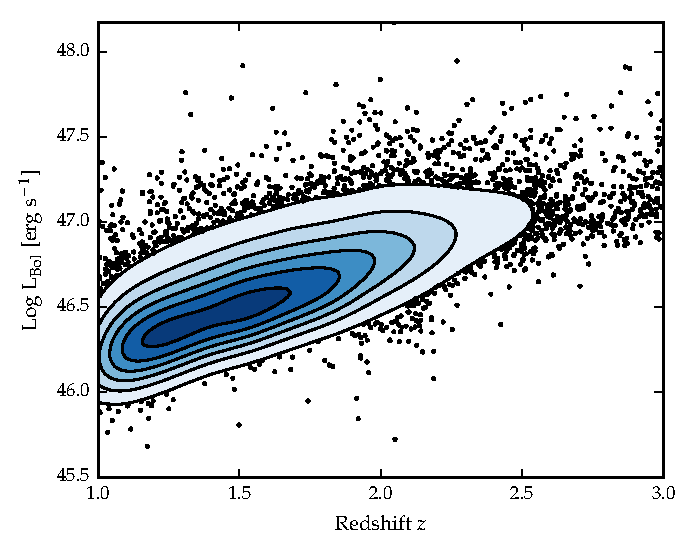
\includegraphics[width=\textwidth]{figures/chapter05/lum_z.pdf}
  \caption[{Distribution of our sample in the redshift-luminosity plane.}]{Distribution of our sample in the redshift-luminosity plane. \todoinline{Just to z=1-3}.}
  \label{fig:lum_z}
\end{figure}

\section{Quasar SED}

Since the physical processes that power AGN are generally understood only qualitatively, almost all AGN SED templates are empirical. 
The empirical template of \citet{elvis94} is still the most commonly cited, despite many additions and updates \citep[e.g.][]{polletta00, kuraszkiewicz03, risaliti04, richards06,  polletta07, lusso10, shang11, marchese12, trichas12}. 
However, these composite spectra are often constructed from quasars with a huge range in luminosity as a function of wavelength. 
In addition, the presence of significant host galaxy at optical wavelengths in low-redshift objects is an additional complication which has not always been taken care of adequately. 
There is therefore a strong rationale for taking a parametric approach to modelling quasar SEDs. 

Our quasars cover the redshift range $0.2 < z < 4$, and so this data covers the rest-frame wavelength range from $800$\,\AA\, to $3.8$\,$\mu$m. 
In this region the SED is dominated by the accretion disc, emission-lines and thermal emission from the hottest (${\mathrm T}\sim1200$K) dust. 
Host galaxy emission is also significant for quasars at redshifts $z\lesssim1$, and the effect of dust extinction at the AGN redshift is another factor which must be considered.   
In this Section, we describe how we have modelled emission from these different physical processes.
Our model is valud between $1216$\,\AA and $3$\,$\mu$m.
At high redshifts, absorption due to Ly-$\alpha$ forest absorption becomes significant. 
Because we do not attempt to model this effect, our model is valid only at wavelengths long-ward of $1216$\,\AA. 
We model dust emission using a single temperature (${\mathrm T}\sim1200$\,K) blackbody, which peaks at $\sim2$\,$\mu$m. 
At longer wavelengths, emission from cooler dust farther from the central engine becomes increasingly important. 
We do not include this emission in our model, which restricts its validity to $\lesssim3$\,$\mu$m.
The model spectrum is shown in Figure \ref{fig:modelsed}, with each of the main components indicated. 

\section{SED Model}

\begin{figure}[h!]
  \centering
  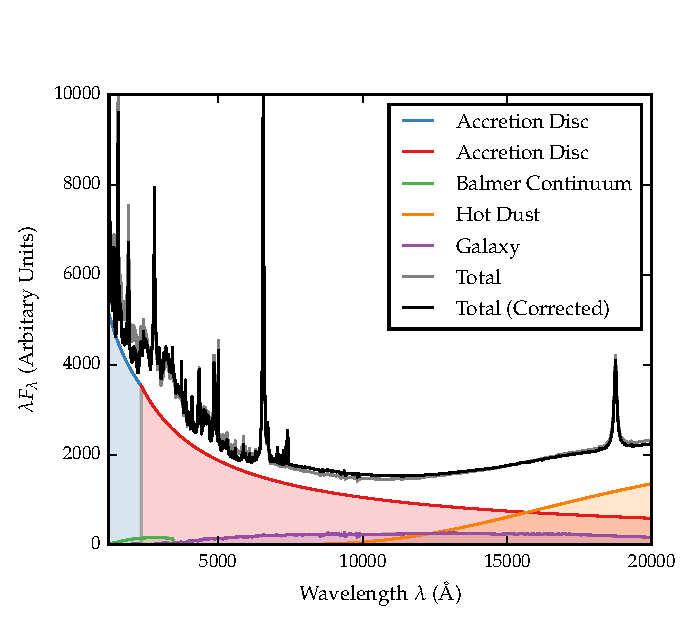
\includegraphics[width=\textwidth]{figures/chapter05/sed_model.pdf}
  \caption[{Model quasar spectrum at $z=1$, showing the contributions to the total flux from the blue power-law slope, red power-law slope, Balmer continuum, blackbody, emission-line spectrum and host galaxy.}]{Model quasar spectrum at $z=1$, showing the contributions to the total flux from the blue power-law slope, red power-law slope, Balmer continuum, blackbody, emission-line spectrum and host galaxy. }
  \label{fig:modelsed}
\end{figure}


\subsection{Accretion Disc}

Thermal accretion disc emission in the $0.1 - 1$\,$\mu$m region is characterised by a broken power-law with three free parameters: a break-wavelength $\lambda_{\mathrm break}$, a blue power-law index $\alpha_{\mathrm blue}$ for wavelengths shorter than the break wavelength, and a red power-law index $\alpha_{\mathrm red}$ for wavelengths longer than the break wavelength.

\subsection{Balmer Continuum}

High order Balmer lines, optically thin Balmer continuum emission, two-photon emission and \ion{Fe}{II} emission blend together to form a distinct feature in quasar spectra at $\sim3000$\AA.
This is referred to as the `Balmer' continuum. 
We simulate the Balmer continuum we use the empirical model given by \citet{grandi82}: 

\begin{equation}
  F(\lambda) = C_{\mathrm BC} \times B_\lambda(T_e)(1-e^{-\tau_\lambda}); \quad \lambda \leq \lambda_{\mathrm BE}
\end{equation}

where $C_{\mathrm BC}$ is a normalisation factor, $B_\lambda(T_e)$ is the Planck function, $T_e=13150$K is the effective temperature, $\lambda_{\mathrm BE}=3460$\AA\, is the wavelength at the Balmer edge, and $\tau_\lambda = \tau_{BE}\left( \nicefrac{\lambda_{BE}} {\lambda} \right)^{-3}$ is the optical depth with $\tau_{\mathrm BE}=45$ the optical depth at $\lambda_{\mathrm BE}$. 
This function is convolved with a Gaussian with $\sigma=5000$\kms to simulate the effect of bulk velocity shifts comparable to those present in broad AGN emission-lines. 

\subsection{Hot Dust}

Thermal emission from hot dust, which dominates the SED at wavelengths longer than $1$\,$\mu$m, is modeled using a blackbody

\begin{eqnarray}  
  F_\lambda = C_{\mathrm BB} \times \frac{2 hc^2}{\lambda^5}\frac{1}{ e^{\frac{hc}{\lambda k_\mathrm{B}T_{\mathrm BB}}} - 1}, 
\end{eqnarray}

with two free parameters: the temperature $T_{\mathrm BB}$ and normalisation $C_{\mathrm BB}$ relative to the power-law continuum. 

\subsection{Emission Lines}

We use an emission-line template taken from \citet{francis91}, which has been extended by \citet{maddox06} to include the \ha and Pa$\alpha$ emission-lines\footnote{The spectrum is not significantly different from the \citet{vandenberk01} SDSS composite}. 
All emission-lines, with the exception of \ha and \hb, are scaled using a single free parameter $C_{\mathrm EL}$, which preserves relative EQWs:

\begin{eqnarray}
  F_{\lambda} =  C_{\mathrm EL} \times \frac{F_{\lambda, \mathrm el}}{F_{\lambda, \mathrm cont}} \times F_{\lambda} 
\end{eqnarray} 

where $F_{\lambda, \mathrm el}$ is the emission-line template, $F_{\lambda,\mathrm cont}$ is the continuum flux in the template, and $F_{\lambda}$ is the continuum flux in the SED model.  
\ha and \hb are scaled separately: 

\begin{equation}
  F_{\lambda} =  C_{\mathrm EL} \times C_{{\mathrm H} \alpha} \times \left( \frac{L(z)} {L(z_{\mathrm nrm})} \right)^{-\beta} \times \frac{F_{\lambda, \mathrm el}}{F_{\lambda, \mathrm cont}} \times F_{\lambda} 
\end{equation}

The luminosity dependence of the \ha EQW (i.e. the Baldwin effect) is parametrised with a power-law with slope $\beta=0.04$.
The redshift dependence of the mean AGN luminosity $L(z)$ for the SDSS quasar catalogue has been determined empirically.

\subsection{Dust Extinction}
\label{sec:sed-extinction} 

The selection criteria of the SDSS DR$7$ quasar catalogue are sensitive to quasars with moderate amounts of dust reddening at the redshift of the quasar, and so we included the effect of dust extinction in our model. 
We use an extinction curve appropriate for the quasar population which has been derived by Paul Hewett. 
To derive the quasar extinction curve, UKIDSS photometry was used to provide an \ebv\footnote{$E(B-V)=A(B)-A(V)$} estimate, via the magnitude displacement of each quasar from the locus of un-reddened objects. 
At redshifts $2 < z < 3$ the reddening measure is made at rest-frame wavelengths $3500-7000$\,\AA, where Galaxy, LMC and SMC extinction curves are very similar. 
The SDSS spectra of the same objects are then employed to generate an empirical extinction curve in the ultraviolet, down to $1200$\,\AA. 
The resulting curve has no $2200$\,\AA\, feature and rises rapidly with decreasing wavelength but is not as steep as the SMC curve. 
The extinctions curves give the colour excess $E(B-\lambda) = A$ relative to the colour excess \ebv as a function of wavelength $\lambda$. 
The colour excess \ebv is related to the extinction in the $V$ band, $A(V)$, via the ratio $R$: 

\begin{eqnarray}
  R_V = \frac{A(V)}{E(B-V)}
\end{eqnarray}

where we assume $R_V = 3$. 
Hence the extinction at a wavelength lambda $A(\lambda)$ is 

\begin{eqnarray}
  A(\lambda) = E(B-V) \times \left[ \frac{E(\lambda-V)}{E(B-V)} + R \right] 
\end{eqnarray}

where the colour excess \ebv is a free parameter in our model. 
The attenuation of the flux at a given wavelength is then:

\begin{eqnarray}
  F_\lambda = F_\lambda10^{-A(\lambda)/2.5}
\end{eqnarray}

in the rest frame of the quasar. 

\section{The `Standard' SED Model} 
\label{sec:ch5-standardmodel}

\begin{figure}
  \centering
  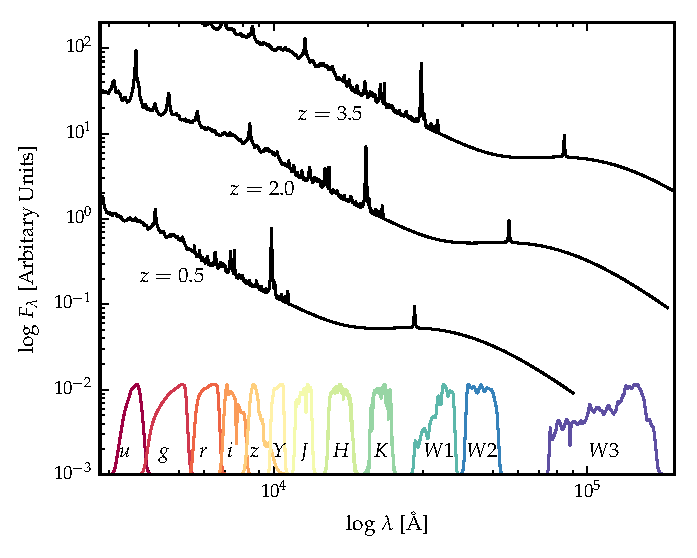
\includegraphics[width=\textwidth]{figures/chapter05/throughput.pdf}
  \caption[{Model quasar spectrum at three different redshifts, and throughput functions for SDSS, UKIDSS and WISE band-passes.}]{Model quasar spectrum at three different redshifts (each arbitrarily scaled), and throughput functions for SDSS, UKIDSS and WISE band-passes.}
  \label{fig:filters}
\end{figure}

We will begin by fitting a single SED model to all $19\,853$ quasars, encompassing a range of redshifts, luminosities, accretion rates etc. 
The free parameters in our model are summarised in Table~\ref{tab:params}. 
The reddening $E(B-V)$ is fixed to zero, since a large fraction of SDSS quasars have very small amounts of dust reddening \citep{richards03}. 
We generate a set of model observed spectra at redshifts from $z=0.25$ to $z=3.75$ in intervals of $\Delta z = 0.1$. 
The SED model is shown at three different redshifts in Figure~\ref{fig:filters}. 

Magnitudes are calculated in the AB system \citep{oke83}, in which case the zero-point flux per unit wavelength is 

\begin{eqnarray}
  \frac{f_\lambda(\lambda)}{{\mathrm erg}~{\mathrm cm}^{-2}~{\mathrm s}^{-1} {\mathrm\AA}^{-1}} = 0.1087 \left(\frac{\lambda}{\mathrm \AA}\right)^{-2}.
\end{eqnarray}


We divide our quasar sample into the same redshift bins.
In each bin we normalise the quasar SEDs in the SDSS $i$ band, and then calculate the median SED. 
The model SED in each redshift bin is similarly normalised. 
The chi-squared statistic is then minimised using the `nelder-mead' algorithm (\todoinline{reference}). 

Our SED model is valid only up to $\lambda \sim 3$\,$\mu$m in the quasar rest frame (the approximate wavelength of the peak in hot dust emission); beyond this additional contributions to the total flux from cooler dust will become significant. 
This prevents us from using the two longest wavelength WISE bands in the fit. 
We also exclude the SDSS $u$ and $g$ band-passes from the fit at $z > 2.7$ and $z > 3.7$ respectively, where these bands start to be affected by Ly$\alpha$ forest absorption.

\section{Results}

The best-fitting parameters from the fit are shown in Table \ref{tab:params}. 
The colours ($r-i$, $i-z$, etc.) of the median SED, the individual quasars, and the best-fitting model are plotted as a function of redshift in Figs.~\ref{fig:color_1} and \ref{fig:color_2}.
Most of the large variations that can be seen in the median colours of the quasars as a function of redshift are due to strong emission-lines being redshifted into and out of the band-passes.
Take away message is that a single, fairly simple parametric is able to reproduce the median colours of tens of thousands of AGN with a large dynamic range in redshift and luminosity. 
However, there is a significant scatter about the median model, which we will investigate in the next Section?
Does any part of this scatter have a systematic dependence on properties of the BH (mass, accretion rate) or outflow diagnostics.  

\begin{table}
  \footnotesize
  \centering
  \begin{tabular}{c c c}
    \hline 
    Parameter & Symbol & Value \\
    \hline 
    Blue power-law index & $\alpha_{\mathrm blue}$ & $-0.478$ \\
    Red power-law index & $\alpha_{\mathrm red}$ & $-0.199$ \\
    Power-law break & $\lambda_{\mathrm break}$ & $2402$ \\
    Blackbody temperature & $T_{\mathrm BB}$ & $1306$\,K \\
    Blackbody normalisation & $C_{\mathrm BB}$ & $2.673$ \\
    Emission-line scaling & $C_{\mathrm EL}$  & $1.240$ \\
    \ha emission-line scaling & $C_{{\mathrm H}\alpha}$  & $0.713$ \\
    Galaxy fraction & $\eta$ & $0.0$ \\
    Balmer continuum scaling & & $0.135$ \\
    \ebv & \ebv & $0.0$ \\

    \hline
  \end{tabular}
  \caption{Model parameters.}
  \label{tab:params}
\end{table}

\begin{figure}
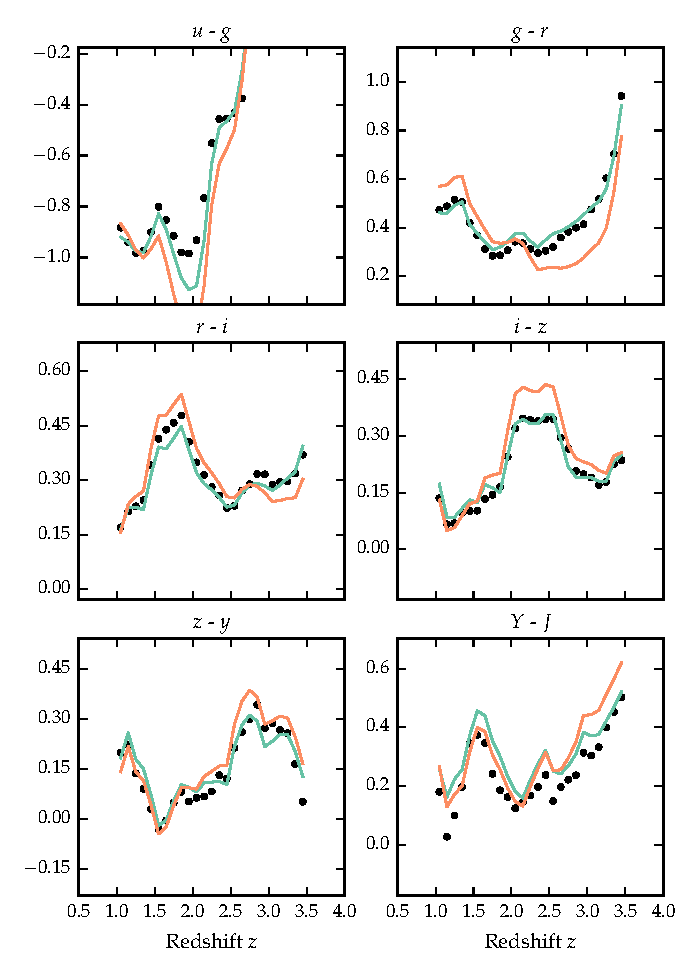
\includegraphics[width=\textwidth]{figures/chapter05/sed_color_plot_1.pdf}
\caption[{Colours of median quasar SED and best-fitting model, with and without correction.}]{Colours of median quasar SED and best-fitting model, with and without correction.}
  \label{fig:color_1}
\end{figure} 


\begin{figure}
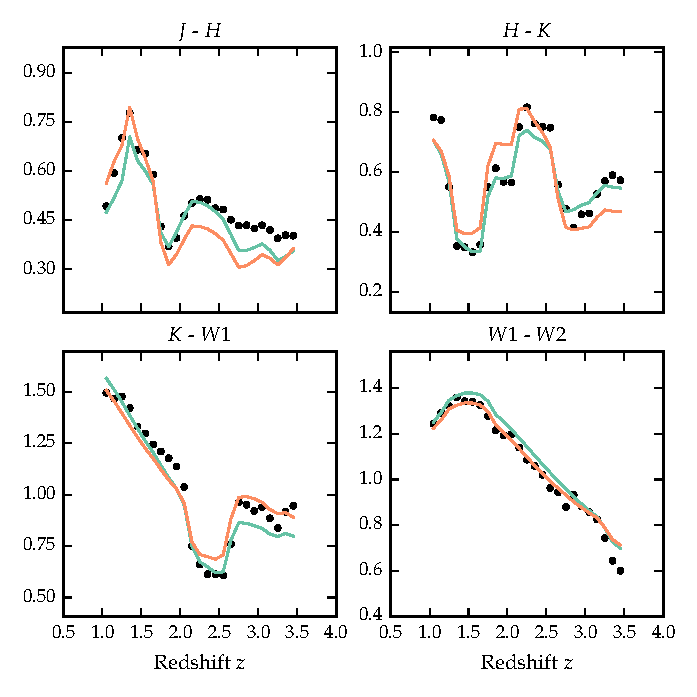
\includegraphics[width=\textwidth]{figures/chapter05/sed_color_plot_2.pdf}
\caption[{Colours of median quasar SED, individual objects, best-fitting  model as a function of redshift.}]{Colours of median quasar SED ({\it black circles}), individual objects ({\it grey points}), best-fitting  model ({\it black line}) as a function of redshift.}
  \label{fig:color_2}
\end{figure} 

\section{Discussion of Fit}

\begin{figure}
  \centering
  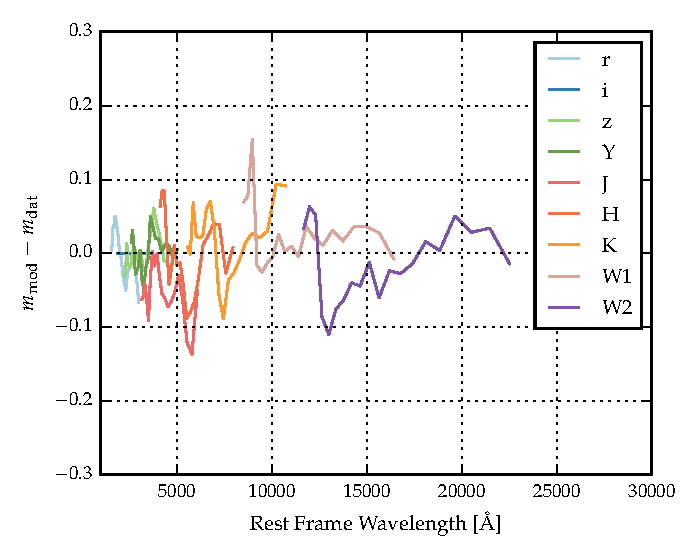
\includegraphics[width=\textwidth]{figures/chapter05/model_residuals.pdf}
  \caption[{Residuals from fit as a function of rest-frame wavelength.}]{Residuals from fit as a function of rest-frame wavelength. \todoinline{Need more info in caption.}}
  \label{fig:residuals}
\end{figure}

In Figure \ref{fig:residuals} we show the difference between the magnitudes from the best-fitting model and the median magnitudes from the sample. 
We have transformed the effective wavelengths of the band-passes to the rest frame of the quasars in each redshift bin, to give the residuals as a function of rest-frame wavelength. 
We represent the residuals measured in each band-pass using a different coloured line. 
Differences between residuals from different band-passes at the same rest-frame wavelength could indicate redshift evolution of the typical quasar SED. 

The residuals indicate that over a large redshift range the model does a fairly good at reproducing the median observed colours of the sample. 
\todo{No: be quantitative}
Most discrepancies are at the $<0.1$\,mag level. 
A single model is effective at reproducing the median colours, suggesting that the properties of a typical quasar do not change significantly over a wide range of redshifts and luminosities. 
\todo{Make sure this is emphasised as a new result.}
One needs to take care in looking at trends with luminosity given the observed-frame band-pass information on the rest-frame SED can produce some strong systematics with redshift, particularly if the SED-model is not a good fit to the actual SED.

\section{Hot Dust}
\label{sec:ch5-hotdust}

\begin{figure}[h!]
\centering
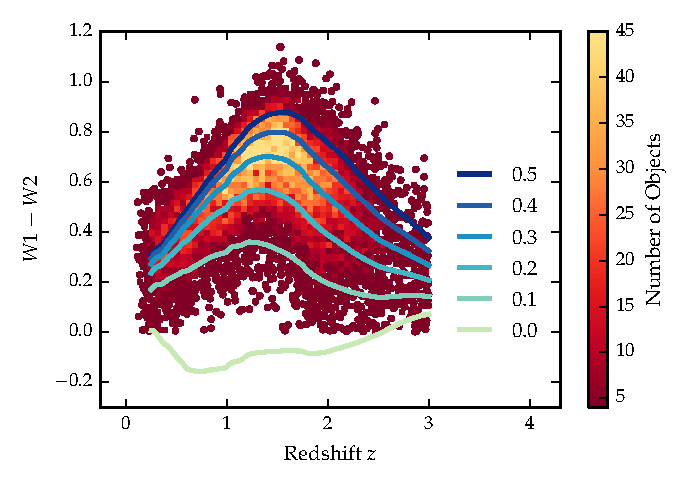
\includegraphics[width=\columnwidth]{figures/chapter05/w1w2_versus_redshift_ratio.pdf}
\caption[{$W1 - W2$ colours of sample as a function of redshift.}]{$W1 - W2$ colours of sample as a function of redshift. Above a density threshold of four points per pixel points are represented by a density plot. On top we plot the colours of our standard SED model, with a fixed temperature and a varying near-infrared ($1 - 3$\,$\mu$m) to ultra-violet ratio.}
  \label{fig:w1w2colorsratio}
\end{figure}

The spread in the $W1W2$ colours (Figure~\ref{fig:w1w2colorsratio}), probing the rest-frame $\sim1-2$\,$\mu$m region, is significant and strongly suggests the presence of real variation in the hot dust temperature and luminosity among the quasars. 

\subsection{Parametrising the hot dust emission}

We characterise the hot dust properties of our sample in terms of the temperature and luminosity of a blackbody.  
We choose to parametrise the luminosity in terms of the near-infrared to ultra-violet luminosity ratio. 
The ultra-violet and near-infrared luminosity are calculated between $2000$ and $9000$\,\AA\, and $1$ and $3$\,$\mu$m respectively.
This is roughly proportional to the covering factor of hot dust ($L_{NIR}/L_{Bol}$) used in some other studies \citep[e.g.][]{roseboom13}. 
The temperature may be related to the distance of the dust from the central engine. 
The value of ($L_{NIR}/L_{Bol}$) is related to the covering factor of the hot dust. 

Some previous studies \citep[e.g.][]{wang13,zhang14} have instead parametrised the near-infrared emission using a power-law ($\propto \lambda^{\beta_{\mathrm NIR}}$), with $\beta \simeq 0.5$. 
We tested this parametrisation, and evaluated it's effectiveness relative to using a blackbody. 
We normalise the power-law at $9000$\,\AA, where its flux is set equal to the flux of the ultra-violet/optical model. 
The near-infrared power-law slope is fit between $\sim1$ and $2.4$\,$\mu$m (with the exact wavelength region being fit depending on the redshift of the quasar). 
We found large residuals in the best-fitting model which varied systematically as a function of $\lambda_{eff}/(1+z)$.  
This suggests that the blackbody is a better fit to the shape of the near-infrared emission than the power-law model \citep[e.g.][]{gallagher07}. 


\subsection{Sample}

Our goal is to determine the temperature and abundance of the hot dust component in individual quasars.  
These properties will be measured by fitting a model to the SDSS-UKIDSS-WISE photometry. 
Constraining a ${\mathrm T}\sim1200$\,K blackbody component in the SED model requires photometric data covering $\sim1-3$\,$\mu$m in the rest-frame of the quasar. 

The observed-frame wavelength coverage of the available band-pass limits the redshift range of the quasars which can be used. 
We consider only quasars at redshifts $z>1$ where the relative host galaxy contribution to the SED is negligible. 
At redshifts $1 \lesssim z \lesssim 1.5$ the available $ugrizYJHKW1W2$ photometry provides good coverage of the rest-frame SED up to $\sim2$\,$\mu$m.
At $z\sim1.5$ the $W2$ band-pass is shifted to $\sim1.8$\,$\mu$m; at higher redshifts $W2$ is probing much shorter wavelengths than the peak of a ${\mathrm T}\sim1200$\,K blackbody. 
Because the shape of the blackbody is not well constrained by the available photometry, the uncertainty on the blackbody temperature measurement increases sharply for quasars at redshifts $z\gtrsim1.5$ 

For the quasars at $z \sim 1$, the WISE $W3$ band is probing rest-frame wavelengths of $\sim5-6$\,$\mu$m. 
This region of the SED is dominated by emission from cooler, more distant dust, which is not accounted for in our model.
However, at redshifts $z \gtrsim 2$ the WISE $W3$ band-pass probes sufficiently short wavelengths to be useful in constraining the shape of the hot blackbody component. 
Therefore, for quasars at redshifts $z > 2$ we again have sufficient constraints from the $ugrizYJHKW1W2W3$ photometry to determine the temperature and normalisation of the blackbody component. 
There are few objects in our sample with redshifts $z > 2.7$, because the SDSS DR7 quasar selection algorithm is highly incomplete at these redshifts.  
Therefore we set $z=2.7$ as the upper limit on the redshift of our sample. 
Because of these constraints, our sample is divided into two parts: one at low redshifts ($1 < z < 1.5$) and the other at higher redshifts ($2 < z < 2.7$). 

We impose a lower-limit signal-to-noise ratio ${\mathrm S/N} > 5$ magnitudes in the $K$, $W1$ and $W2$ band-passes for the low-$z$ sample and ${\mathrm S/N} > 5$ in the $W1$, $W2$, and $W3$ band-passes for the high-$z$ sample to ensure reliable photometry.
This gives us $5\,910$ quasars in our low-$z$ sample and $1\,989$ quasars in our high-$z$ sample. 

\begin{table}
  \footnotesize
  \centering
  \begin{tabular}{cccc}
    \hline 
    Sub-sample & Number of AGN & Data & Redshift range \\
    \hline 
    Low-$z$ & 5,910 & $ugrizYJHKW1W2$ & $1 < z < 1.5$ \\
    High-$z$ & 1,989 & $ugrizYJHKW1W2W3$ & $2 < z < 2.7$ \\           
    \hline
  \end{tabular}
  \caption{Summary of sub-samples.}
  \label{tab:sub-samples}
\end{table}


We will hold most model parameters fixed, and vary only the blackbody parameters which parametrise the near-infrared emission. 
Therefore, we need to define a sub-sample of objects which we know are well fit by our standard SED model in the ultra-violet/optical region. 
This means excluding objects with extreme emission-line EQWs and/or significant dust extinction.
We use the $i-K$ colours of the quasars as a measure of the overall colour of the quasars as it provides the longest baseline in wavelength without being affected by absorption in the Ly$\alpha$ forest at high redshifts. 
This is shown in Figure~\ref{fig:ikzplot}.
A significant amount of the scatter in $i-K$ can be attributed to intrinsic variations in the ultra-violet power-law slopes of the individual quasars, which is why we allow a negative reddening. 
The SDSS and UKIDSS photometry are separated by $3-4$ years in the source rest-frame. 
Therefore, some of the $i-K$ scatter could be due to temporal variations in the brightness of the targets. 
However, the red-asymmetry of the $i-K$ colours about the un-reddened SED model suggests that this effect is sub-dominant to intrinsic colour differences. 
However, there is a clear `red tail' to the colour distribution which can be explained by dust reddening at the redshift of the quasar.
We discarded from our sample quasars with $i - K$ colours redder than our standard model with dust reddening \ebv $= 0.075$ and bluer than \ebv $=-0.075$ (Figure~\ref{fig:ikzplot}). 
Following this cut we are left with $4\,615$ quasars in our low-$z$ sample and $1\,692$ quasars in our high-$z$ sample. 

\begin{figure}
  \centering
  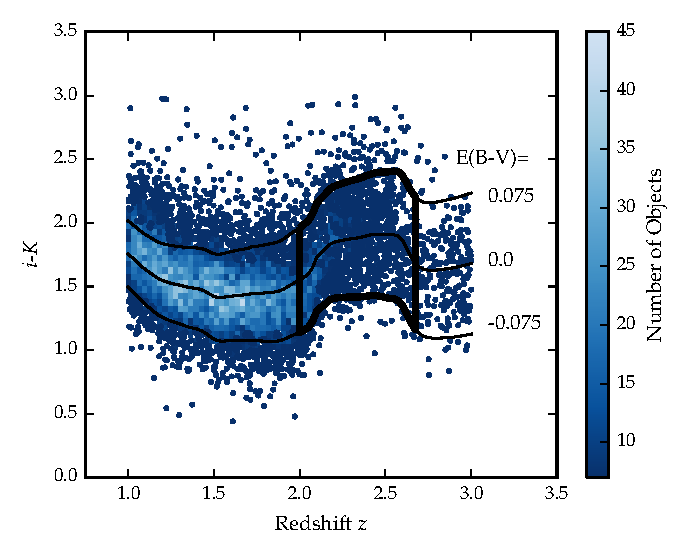
\includegraphics[width=\columnwidth]{figures/chapter05/ik_versus_z_low_ext.pdf}
  \caption[{$i-K$ colours of non-BAL DR7Q quasars with $i>19.1$ as a function of redshift.}]{$i-K$ colours of non-BAL DR$7$Q quasars with $i>19.1$ as a function of redshift. The lines show the colours of our model with varying amounts of dust extinction. Quasars with extinction $|E(B-V)|>0.075$ are excluded.}
  \label{fig:ikzplot}
\end{figure}

\subsection{Diversity in hot dust properties}

In Figure~\ref{fig:w1w2colorsratio} we plot the $W1 - W2$ colours of the sample as a function of redshift at $z<3$. 
In this redshift range the $W1$ and $W2$ band-passes are probing the $1.2 - 2.8$\,$\mu$m and $1.6 - 3.8$\,$\mu$m region of the rest frame SED respectively. 
For reference, the peak wavelength is at $2.4$\,$\mu$m for a blackbody radiating at $1200$\,K. 
At any given redshift we see a $\sim 0.5$\,mag dispersion in the $W1-W2$ colours. 

On the same axes in Figure~\ref{fig:w1w2colorsratio} we have plotted the $W1-W2$ colours derived from our SED model with a fixed blackbody temperature ($1216$\,K) and a ratio of near-infrared to ultra-violet luminosity ranging from $0.0$ to $0.5$, with the other model parameters held constant. 
We conclude that even with the sample restricted to be uniform in its ultra-violet/optical properties, we still get an significant spread in $W1-W2$ colours, which we can use to learn about the diversity of near-infrared properties in our sample. 
In the rest of this Chapter we will characterise the hot dust properties of our sample, and test its relation to quasar properties such as luminosity, black-hole mass and normalised accretion rate, and outflow-properties. 

\section{Fitting procedure}

We will fit a model to the individual quasar SEDs, allowing the temperature and normalisation of the black body component to vary. 
The model spectrum is redshifted to the redshift of the quasar being fit and is then multiplied by the $ugrizYJHMW1W2W3$ throughput functions and normalised appropriately to give AB magnitudes. 
We minimise the chi-squared statistic using the minimisation is done using the 'nelder-mead' algorithm.
To avoid significant absorption in the Ly$\alpha$ forest at high-$z$, we restrict our fitting to wavelengths greater than $2000$\,\AA; when the effective wavelength of a band-pass falls below this limit the band-pass is excluded from the fit. 
\todo{2000A is quite large given the Ly-alpha forest impacts from 1216A.}
$W3$ is only used for the quasars at redshifts $2 < z < 2.7$. 

\section{Results}

\todo{Show some example fits? Show overlayed data/model with alpha=0.1? e.g. figures/chapter05/ntt\_proposal\_figure2.pdf}

In Figure~\ref{fig:ratio_tbb_density} we see that the two parameters are clearly correlated. 
For a lower temperature blackbody the near-infrared to ultra-violet luminosity ratio is larger. 
Such a correlation is to be expected: as the blackbody temperature is lowered, the peak shifts to longer-wavelengths (following Wien's displacement law). 
Because of this degeneracy we need to be very careful to separate out real trends of $R_{NIR/UV}$ with other quasar properties from indirect trends resulting from a mutual dependence on $T_{BB}$.  

\begin{figure}[h!]
  \centering
  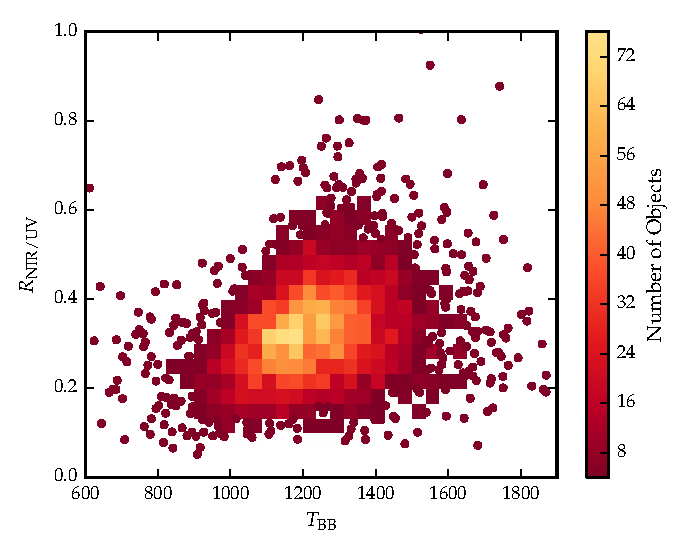
\includegraphics[width=\textwidth]{figures/chapter05/ratio_tbb_density.pdf}
  \caption[{Ratio of near-infrared to ultra-violet luminosity ($R_{NIR/UV}$) against temperature ($T_{BB}$) for low-$z$ sample.}]{Ratio of near-infrared to ultra-violet luminosity ($R_{NIR/UV}$) against temperature ($T_{BB}$) for low-$z$ sample. The density of points is shown in more dense regions of the space, and individual objects in less dense regions.}
  \label{fig:ratio_tbb_density}
\end{figure}

In Figure~\ref{fig:ratio_tbb_density} we show that there is significant range of temperature and normalisation present in our sample. 
However, we need to quantify  how much of this is due simply to uncertainties in the fits stemming from uncertainties in the photometry. 
In order to achieve this we took our standard SED model with a single temperature and normalisation blackbody component, and generated $200$ mock SEDs with a brightness distribution similar to that of our real sample. 
We estimated the mean uncertainty of the magnitudes in the $K$, $W1$, and $W2$ band-passes as a function of apparent brightness. 
We then sampled the $K$, $W1$, and $W2$ magnitudes from Gaussian distributions, with a mean equal to the magnitude of the model SED, and the width equal to the mean uncertainty at the appropriate brightness. 
Finally, we fit these mock SEDs using our standard fitting procedure. 
The results are shown by the red points in Figure~\ref{fig:ratio_tbb_density}
We can see that scatter introduced by the uncertainty in the photometry is significantly less than the intrinsic scatter in the data. 
This demonstrates that there is a real distribution of hot dust temperatures and luminosities in our sample. 

\subsection{Correlations with quasar properties}

\begin{figure}
  \centering
  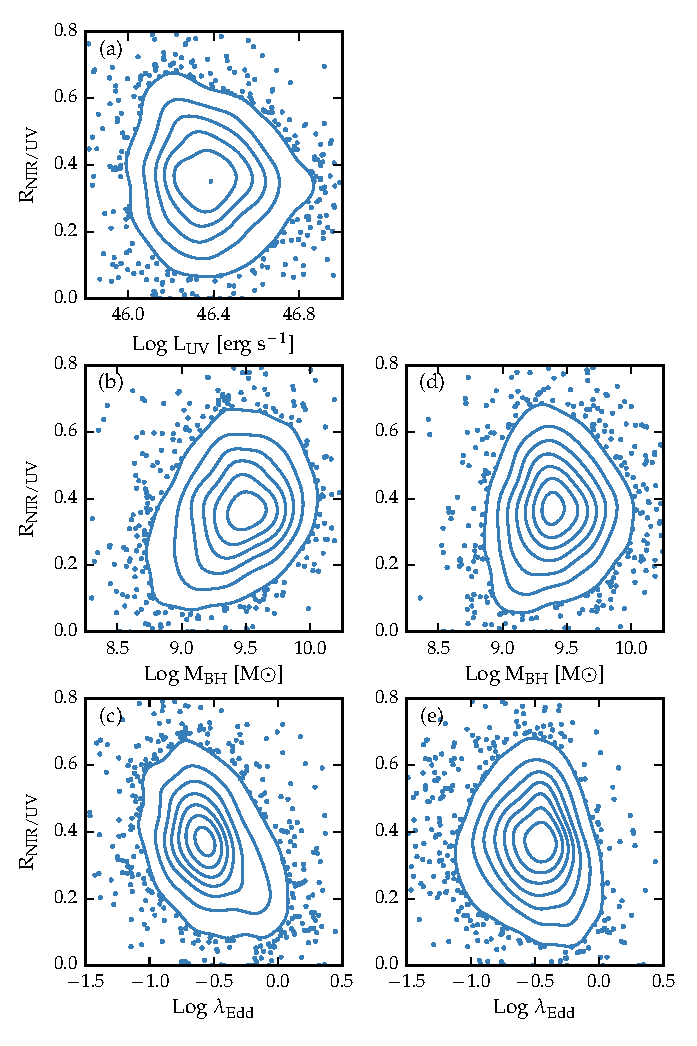
\includegraphics[width=\textwidth]{figures/chapter05/correlations_contour.pdf}
  \caption[{Best-fit blackbody temperature against ultra-violet luminosity, black-hole mass and Eddington ratio.}]{Best-fit blackbody temperature against ultra-violet luminosity (left), black-hole mass (centre) and Eddington ratio (right) for $1 < z < 1.5$ sample (black) and $2 < z < 2.7$ sample (black).}
  \label{fig:correlations_contour}
\end{figure}

We now look for correlations between the properties of the blackbodies we have fitted to the hot dust emission and other properties of the quasar such as redshift, BH mass, normalised accretion rate (Eddington ratio), and outflow diagnostics.  
\todo{Calculate new BH masses and redo this section.}

There is a clear anti-correlation between the ultra-violet luminosity and the best-fit blackbody temperature. 
We calculated a Spearman rank-order correlation coefficient $-0.33$. 
\todo{Do we believe this trend is real?}
\todo{This is just for low-z sample.}
The black-hole masses are virial estimates calculated by Shen et al. 2011 using the MgII emission-line in the SDSS spectra. 
The Eddington ratios (bolometric luminosity normalised by Eddington luminosity) are also calculated by Shen et al. 2011 using bolometric corrections in Richards et al. (2006a) using 3000\AA monochromatic luminosities. 
There are no significant correlations between $T_BB$ and $R_{NIR/UV}$ and the ultra-violet luminosity, black-hole mass or Eddington ratio. 

The dynamic range in luminosity is very limited. 
I will combine the low and high $z$ samples. 
As first step see if there is a difference in the median $R_{NIR/UV}$ for low/high luminosity samples. 

At low-$z$  we get a much larger range in blackbody temperatures from our fits. 
We discussed how the W3 S/N > 5 cut might be be biasing the high-z sample if the subset being removed had properties distinct from the remainder of the sample. 
The W3 S/N > 5 cut removes about 25 per cent of the sample. 

We observe a positive correlation between the black-hole mass and the near-infrared to ultra-violet luminosity ratio which is quite different from what we observed in our low-$z$ sample. 
We believe that this is just a manifestation of the fact that at high redshift the black-hole masses are derived from CIV. 
We will show below how the FWHM of CIV has a positive correlation with the hot dust abundance, and large CIV FWHM leads to larger black hole mass estimates. 
This explains the apparent correlation between the IR/ultra-violet ratio and the black hole mass. 
Eddington ratio measures the luminosity relative to the Eddington luminosity. 
Higher BH mass estimates will lead to lower Eddington ratios, which is why the Eddington ratio appears to decrease with increasing IR/ultra-violet ratio. 
For the sources in our low-$z$ sample the black-hole mass is measured using the broad MgII emission-line. 
As we will show below, the properties of the MgII emission-line have no dependence on the hot dust properties. 


\subsubsection{Composite spectra}

\begin{figure}
  \centering
  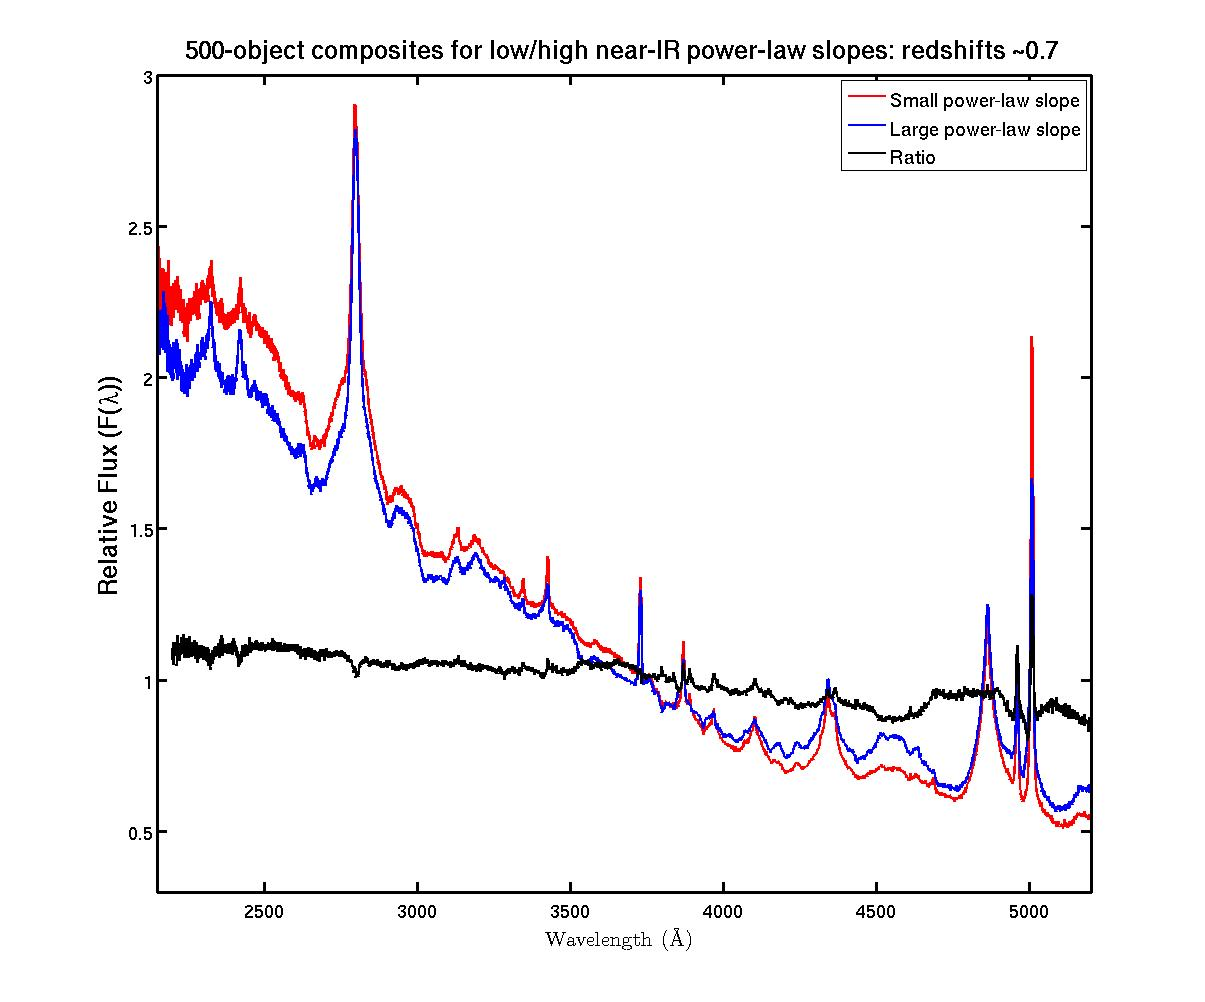
\includegraphics[width=\textwidth]{figures/chapter05/z07_pls_comps.jpg}
  \caption[{Composite SDSS spectra for objects at $z\sim0.7$.}]{Composite SDSS spectra for objects at $z\sim0.7$. We have divided sample into objects with objects best-fit by small (red line) and large (red line) values of $\beta$. \todoinline{Remake if possible}.}
  \label{fig:pls_comp}
\end{figure}

Is there a connection between the hot dust properties and EV1? 
To test this we can divide the quasar sample by hot dust properties, and then generate composite spectra. 
The EV1 original EV1 correlates - \ion{Fe}{II}, \hb, [\ion{O}{III}] - are at around 4000-6000\AA. 
The SDSS spectra are probing shorter wavelengths at redshifts $z\gtrsim1$.
Recall that our sample does not include any quasars at redshifts $z<1$, where the host galaxy emission starts to become significant. 
\todo{Need to decide what to do here. If I say host galaxy is significant using the power-law slope won't help. Use blackbody fits instead?}

The $z < 0.8$ SDSS spectrum composite comparison for the small and large $\beta_{NIR}$ sub-samples (Figure~\ref{fig:pls_somp}) is a very direct illustration of EV$1$. 
Hot dust emission increases with \ion{Fe}{II} EW. 
We also note that the amount of hot dust correlates with the \ion{Si}{III}/\ion{C}{III}] emission ratios. 
The \ion{Si}{III}/\ion{C}{III}] ratio is generally considered to be a good indicator of density and is one of the primary EV1 correlates. 
The relative flux ratio of \ion{Si}{III} to \ion{C}{III}] increases when \ion{C}{IV} is more blue-shifted \citep{richards11}. 
The \ion{Mg}{II} emission-line has exactly the same profile/shape for the two samples (apparent changes in \ion{Mg}{II} seen in Figure~\ref{fig:pls_comp} are the result of changes in \ion{Fe}{II} at wavelengths just short-ward of the line). 
Finally, we note that objects with more hot dust are slightly redder.

\citet{shen14} also find that torus emission is enhanced in quasars with larger $R_{FeII}$.
They suggests that this may be caused by more efficient disc winds that facilitate the formation of a dusty torus. 

\subsubsection{High-$z$}

In Figure~\ref{fig:civ_hot_dust} we show how the ratio of near-infrared to ultra-violet luminosity depends on the blueshift and rest-frame EQW of the \ion{C}{IV} line.
\ion{C}{IV} blueshifts are calculated as in Section XX. 
We see that the near-infrared to ultra-violet luminosity ratio is strongly correlated with the blue-shift of the \ion{C}{IV} emission-line. 
A similar trend was noted by \citet{wang13}. 
Interestingly, we note strong similarities to the object subsets selected according to their \ion{C}{IV}-emission properties in \citet{richards11} (see Figures 11 \& 12).  
We note that the correlation between the hot dust and the \ion{C}{IV} emission properties will lead to apparent correlations between the host dust and the BH mass. 
 
\begin{figure}
\centering
  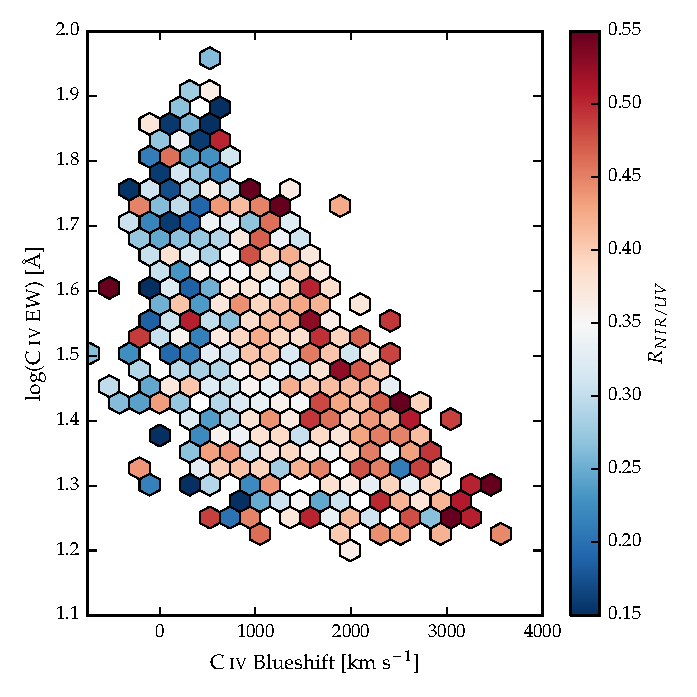
\includegraphics[width=\columnwidth]{figures/chapter05/hot_dust_ratio.pdf}
\caption[{Hot dust abundance as a function of rest-frame EQW and blueshift of the \ion{C}{IV} line.}]{Rest-frame EQW and blueshift of the \ion{C}{IV} line for XX SDSS DR7 quasars. The colours of the hexagons denote the median hot dust (T$\simeq$1200\,K) abundance for all quasars at a given EQW and blueshift. Quasars with the most extreme outflow signatures are predominantly hot-dust rich. Only bins containing a minimum of two objects are plotted. \citet{hewett10} redshifts are adopted to calculated \ion{C}{IV} blueshifts.}
  \label{fig:hot_dust_beta}
\end{figure}

\begin{figure}
\centering
  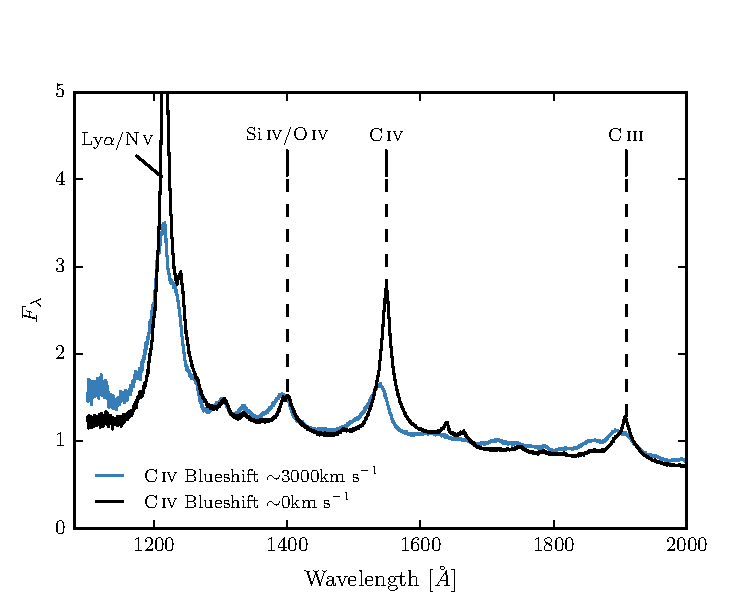
\includegraphics[width=\columnwidth]{figures/chapter05/blueshift_composite.pdf}
\caption{}
  \label{fig:blueshift_composite}
\end{figure}




\section{Discussion}

R isn't necessarily the total mass of hot dust, but more the covering factor of hot dust and the area which is intercepted by our line of sight. 
Ultra-violet photons from the accretion disc accelerate the wind via radiation line driving.
Dust absorption contributes to the outflow acceleration. 
Wind could be driven by radiation pressure on dust grains. 
For an AGN radiating at 0.1Ledd radiation pressure is sufficient to unbind dust from the gravitational porential (e.g. Pier \& Krolik 1992; Honig \& Beckert 2007). 
It would be efficiently accelerated by the central continuum source because of the high cross-section of dust \citep[e.g.][]{fabian12}.  
That flattens the geometry of the wind and exposes more surface area that is viewable on a relatively face-on line of sight.  
The radiation pressure is increased at higher luminosities and/or accretion rates.
This can flatten the geometry of the wind, thereby increasing the range of angles for which the inner edge of the dusty wind - where dust is at it's sublimation temperature - can be observed. 
A direct prediction is therefore that the in a quasars with high accretion rates and strong outflows, the emission from hot dust should be enhanced. 
(See Kishimoto picture)
Also maybe supported by Roseboom - strong anti-correlation between torus covering factor and hot dust. as the covering factor of the torus decreases, the maximum inclination at which a type 1 quasar would be seen increases. 
An increase in the inclination will mean direct sight lines to more of the inner wall of obscuring material closest to the accretion disc. 
\citet{roseboom13} studied a similar sample of luminous type 1 quasars. 
They, like us, modelled the near-infrared emission using a blackbody and modelled the emission at longer wavelengths using a clumpy torus model. 
They find that while $L_{1-5\mu m}$/$L_{IR}$ appears relatively insensitive to $L_{bol}$ and $L_{IR}$, a strong correlation appears between $L_{1-5\mu m}$/$L_{IR}$ and $L_{IR}/L_{bol}$ (i.e. the dust covering factor). 
They explain this correlation by postulating that as the covering factor of the torus decreases, the maximum inclination at which a type 1 quasar would be seen increases. 
An increase in the inclination will mean direct sight lines to more of the inner wall of obscuring material closest to the accretion disc.

\citet{wang13}, fitting the near-infrared emission with a single power-law, found that objects with strong outflow signatures (blueshift and asymmetry index (BAI) and full width at half-maximum (FWHM) of CIV) have more hot dust emission relative to the accretion disc emission in a large sample of $z\sim2$ non-BAL quasars. 
Also found by \citet{shen14}. 
Compared to Wang we have larger sample, better blueshift meaurements (try use ICA?) and use blackbody (find power-law poor fit), data from UKIDSS, full sed model

At lower redshifts, \citet{shen14} have found that the hot dust properties are correlated with EV$1$. 
\citet{shen14} quantify the relative torus emission using the $r-W1$ colour for a sample of $0.4 < z < 0.8$ SDSS quasars. 
At these redshifts $W1$ is observing between $1.9$ and $2.4$\,$\mu$m in the rest-frame of the quasar, which suggests that they are sensitive to the same component of hot dust which we are investigating. 
Restrict redshift range t limit effect of band shifting due to redshift. 
Relative high flux in in the infrared than in the optical as Eddington ratio increases. 

